\documentclass{article}
\usepackage[english, provide=*]{babel} % Changed from 'english' to 'american'
\usepackage{amsmath}
\usepackage{graphicx}
\usepackage{hyperref}

\title{Assigment 2}
\author{Nguyen The Binh - ITCSIU23003\\Instructor: Le Thi Ngoc Hanh (Ph.D)}

\date{\today}


\begin{document}
\maketitle

\section*{1. Usecase Diagram}
Below is the usecase diagram for the A Restaurant Reservation System RRS
\subsection*{}
\begin{figure}[h]
  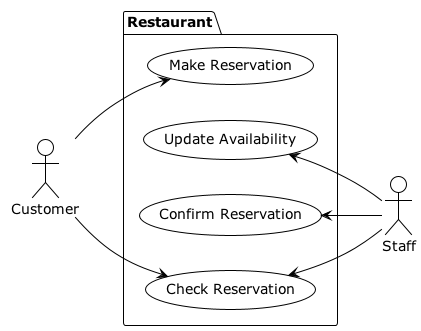
\includegraphics[scale=0.5]{out/usecase/usecase.png}
  \centering
  \caption{Usecase diagram}
  \centering
\end{figure}
TODO: write explanation

\clearpage % Insert a page break here


\section*{2. Activity Diagram}
I have selected the Make Reservation usecase for creating a activity diagram, which is shown below.
\subsection*{}
\begin{figure}[h]
  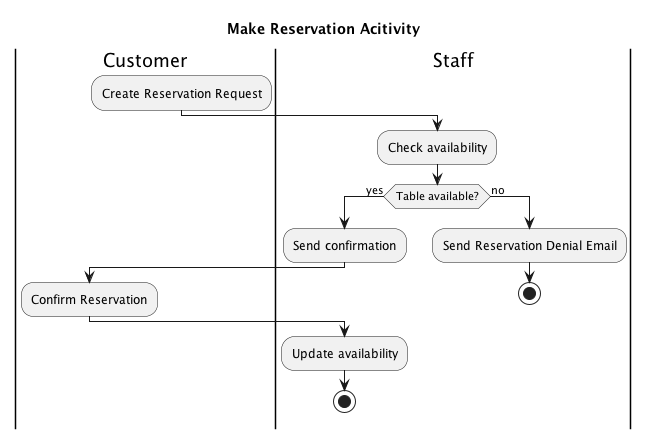
\includegraphics[scale=0.5]{out/RRS_activity/RRS_activity.png}
  \centering
  \caption{Activity diagram for make Reservation}
  \centering
\end{figure}
TODO: write explanation

\clearpage
\section*{3. Participants of Scenario}
In The case of Table is available for reservation, we can see the collaboration between the Customer
and Staff of the Restaurant

\begin{itemize}
  \item Staff: Create and send confirmation email to Customer, wait for confirmation. Update availability if Reservation is confirmed
  \item Customer: Confirm the reservation.
\end{itemize}

\end{document}